\documentclass{article}
% Chinese
% \documentclass[UTF8, nofonts, mathptmx, 12pt, onecolumn]{article}
% \usepackage{xeCJK}
% \setCJKmainfont{SimSun}
\usepackage{amsmath}
\usepackage{amsfonts}
\usepackage{amssymb}
\usepackage{wasysym}
% \usepackage{ctex}
\usepackage{graphicx}
\usepackage{float}
\usepackage{geometry}
\geometry{a4paper,scale=0.8}
\usepackage{caption}
\usepackage{subcaption}
% \newcommand{\oiint}{\mathop{{\int\!\!\!\!\!\int}\mkern-21mu \bigcirc} {}}
\newcommand*{\dif}{\mathop{}\!\mathrm{d}}
\newcommand*{\md}{\mathop{}\!\mathrm{d}}
\newcommand*{\me}{\mathrm{e}}

% \usepackage{parskip}
% \setlength{\parindent}{0cm}

\usepackage{bm}
\let\Oldmathbf\mathbf
\renewcommand{\mathbf}[1]{\boldsymbol{\Oldmathbf{#1}}}
\let\eqnarray\align

\author{Xiping Hu}
\usepackage{authblk}
\author{Xiping Hu}
\affil{http://thehxp.tech/}
\title{Homework for Chapter 2}

\begin{document}
\maketitle

\begin{figure}[H]
  \centering
  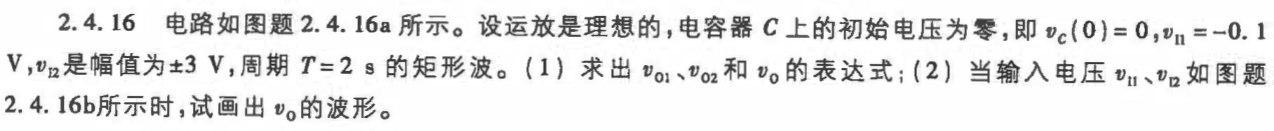
\includegraphics[width=\linewidth]{figures/Problem4-1}
  \label{fig:}
\end{figure}
\begin{figure}[H]
  \centering
  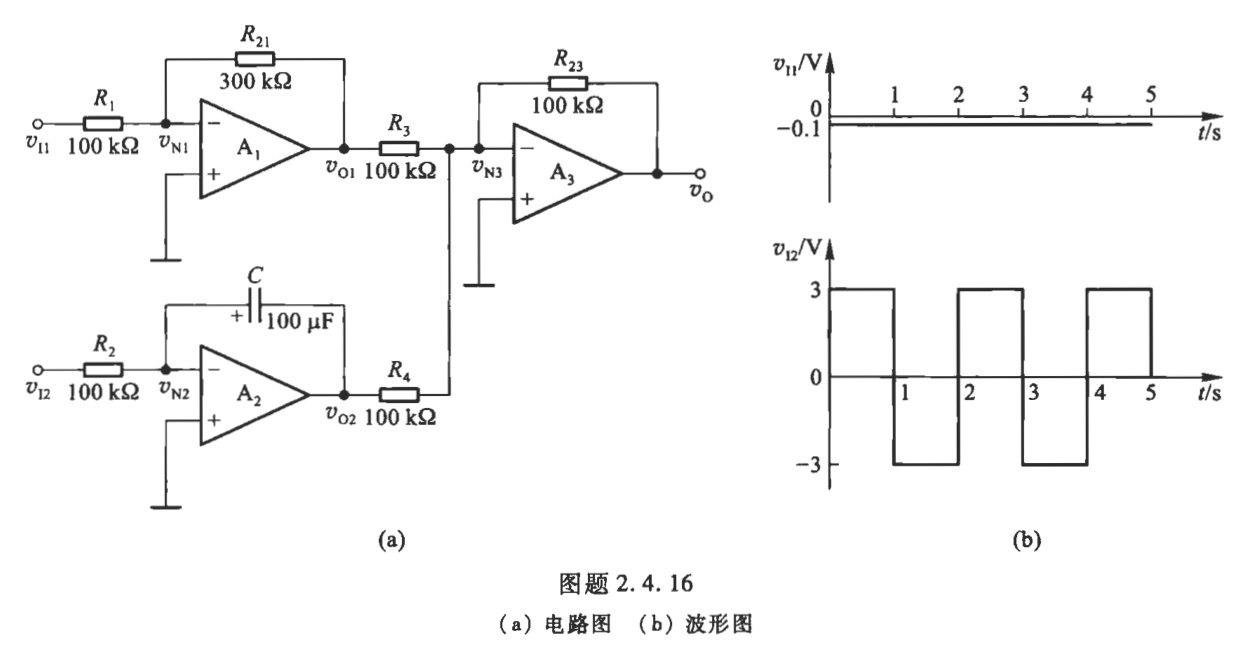
\includegraphics[width=\linewidth]{figures/Problem4-2}
  \label{fig:}
\end{figure}

\paragraph{Solution}

\begin{equation*}
  \begin{aligned}
    v_{o1} &= - \dfrac{R_{21}}{R_1} v_{I1} = 0.3 \  \mathrm{V} \\
    v_{o2} &= - \dfrac{1}{R_2 C} \int_0^t v_{I2} \md t = - \dfrac{1}{10} \int_0^t v_{I2} \md t 
  \end{aligned}
\end{equation*}

\begin{equation*}
  \begin{aligned}
    v_o &= - \left( \dfrac{R_{23}}{R_3} v_{o1} + \dfrac{R_{23}}{R_4} v_{o2}   \right) \\
    &= \dfrac{R_{21} R_{23}}{R_1 R_3} v_{I1} + \dfrac{R_{23}}{R_2 R_4 C} \int_0^t v_{I2} \md t \\
    &= -0.3 + \dfrac{1}{10} \int_0^t v_{I2} \md t 
  \end{aligned}
\end{equation*}

This figure below shows how $v_o$ varies with time.

\begin{figure}[H]
  \centering
  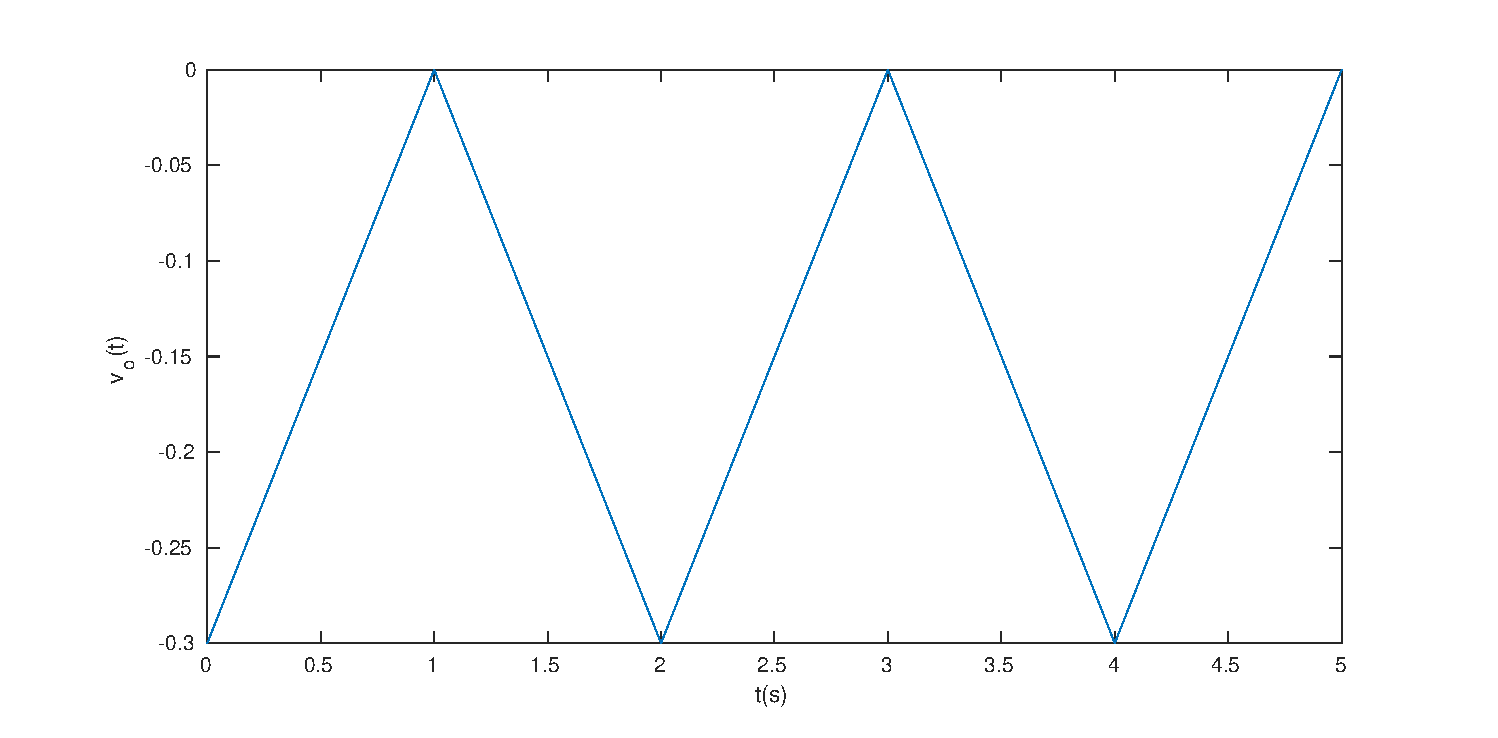
\includegraphics[width=\linewidth]{figures/Problem4-3}
  \label{fig:}
\end{figure}



\end{document}